\documentclass[12pt,a4paper]{article}
\usepackage{amsmath,amssymb,amsthm}
\usepackage{hyperref}
\usepackage{listings}
\usepackage{geometry}
\usepackage{graphicx}
\geometry{margin=1in}

\title{The True String \(T\): A Collision-Zero Encoding via \(f(m,n)=4+3m+3n+2mn\)}
\author{Gabriel Christensen}
\date{\today}

\newtheorem{definition}{Definition}[section]
\newtheorem{lemma}{Lemma}[section]
\newtheorem{theorem}{Theorem}[section]
\newtheorem{corollary}{Corollary}[section]

\begin{document}

\maketitle
\begin{abstract}
We define a collision-zero mapping based on the bivariate form \(f(m,n)=4+3m+3n+2mn\) over nonnegative integers and study the resulting set-valued structure. We formalize the encoding, analyze zero vs. unique occurrences, and provide computational methods to verify properties. We discuss relationships to classical prime distributions. This model is empirical and does not constitute a proof of the Riemann Hypothesis; any RH-related content is observational only.
\end{abstract}

\tableofcontents
\newpage

\section{Introduction}
We consider a self-referential encoding in which repeated images cancel to zero. The purpose is to study multiplicity and prime occurrences within the image of \(f\), not to claim full coverage of all integers.

\section{Preliminaries and Definitions}
\begin{definition}[Generating form]\label{def:f}
For \(m,n\in\mathbb{N}_0\) define
\[
 f(m,n) = 4 + 3m + 3n + 2mn.
\]
\end{definition}

\begin{definition}[Collision-zero structure \(T\)]\label{def:T}
Initialize an empty map \(T\). For each \((m,n)\), compute \(x = f(m,n)\).
\begin{itemize}
    \item If \(x\notin T\), set \(T[x]=x\).
    \item If \(x\in T\), set \(T[x]=0\) to indicate a collision.
\end{itemize}
\end{definition}

\begin{definition}[Zeros and prime elements]
Elements with \(T[x]=0\) are \emph{zeros} (collisions). Elements with \(T[x]=x\) and \(x\) prime are \emph{prime elements}.
\end{definition}

\subsection*{Notation}
We write \(\mathbb{N}_0=\{0,1,2,\dots\}\). For an odd integer \(c\ge 1\), let \(d_{\mathrm{odd}}(c)\) denote the number of odd divisors of \(c\) (including \(1\) and \(c\)).

\begin{center}
\begin{tabular}{l l}
Symbol & Meaning \\
\hline
\(\mathbb{N}_0\) & Nonnegative integers \\
\(f(m,n)\) & \(4+3m+3n+2mn\) \\
\(F(m,n)\) & Same as \(f\); used in coverage/multiplicity section \\
\(T[x]\) & Collision-zero value at index \(x\) (0 if repeated) \\
\(d_{\mathrm{odd}}(c)\) & Number of odd divisors of odd \(c\) \\
\end{tabular}
\end{center}

\section{Basic properties}
\begin{lemma}[Collision encoding]\label{lem:collision}
For any \(x\), \(T[x]=0\) iff there exist distinct pairs \((m_1,n_1)\ne(m_2,n_2)\) with \(f(m_1,n_1)=f(m_2,n_2)=x\).
\end{lemma}

\begin{lemma}[Modulo-3 image]\label{lem:mod3}
For all \(m,n\in\mathbb{N}_0\), \(f(m,n) \equiv 1 + 2mn \pmod{3}\). As \(mn\) ranges over \(\{0,1,2\}\pmod{3}\), the image attains all residue classes \(0,1,2\pmod{3}\). In particular, values congruent to \(2\pmod{3}\) occur when, e.g., \(m\equiv 1\) and \(n\equiv 2\) (or vice versa) modulo 3.
\end{lemma}

\begin{remark}[Empirical sparseness]\label{rem:sparse}
The image of \(f\) is a strict subset of \(\mathbb{N}\), and empirical data suggest nontrivial distributional structure (see Section on residue profiles). We do not make density claims here.
\end{remark}

\section{Computational methods}
We provide a generator script \texttt{python/true\_string\_collision.py} that enumerates values of \(f\) over a rectangle \([0,M]\times[0,N]\), counts collisions, and classifies unique outputs as prime/non-prime.

\begin{lstlisting}[language=bash,caption=Example usage]
python3 python/true_string_collision.py --max-m 200 --max-n 200 --list-first 20
\end{lstlisting}

\section{Empirical residue profiles}
We report residue distributions among distinct outputs of \(f\) and small-prime divisibility counts, produced by:\\
\texttt{python3 python/true\_string\_collision.py --max-m 120 --max-n 120 --mods 3,4,8 --divisible-by 2,3,5,7,11}

For \(m,n\le 120\) (distinct outputs = 5854), the residue counts were:
\begin{center}
\begin{tabular}{l|rrrrrrrr}
Mod & r0 & r1 & r2 & r3 & r4 & r5 & r6 & r7 \\
\hline
3 & 1513 & 2859 & 1482 & -- & -- & -- & -- & -- \\
4 & 1491 & 1457 & 1452 & 1454 & -- & -- & -- & -- \\
8 & 743 & 729 & 728 & 727 & 748 & 728 & 724 & 727 \\
\end{tabular}
\end{center}

Divisibility among distinct outputs (same run):
\begin{center}
\begin{tabular}{l|rrrrr}
Prime & 2 & 3 & 5 & 7 & 11 \\
\hline
Count & 2943 & 1513 & 1018 & 759 & 503 \\
\end{tabular}
\end{center}

These profiles are parameter-dependent and intended as empirical summaries to guide further analysis.

\subsection*{Figures}
If generated via the plotting script, figures are saved under \texttt{fig/}. For example (for \(m,n\le 120\)):
\begin{figure}[h]
\centering
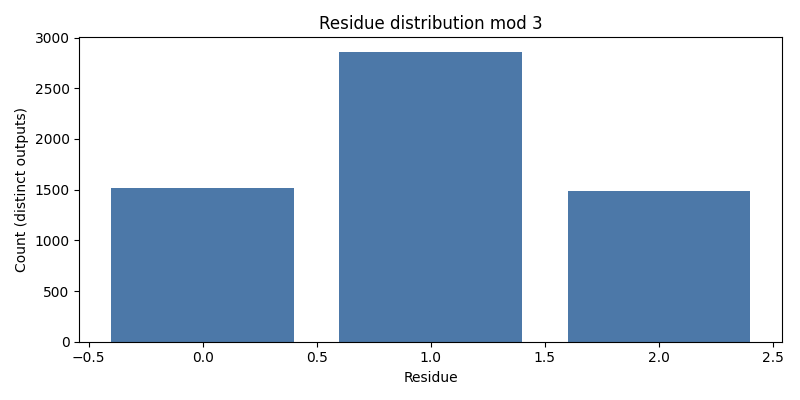
\includegraphics[width=0.7\linewidth]{../fig/residues_mod_3.png}
\caption{Residue distribution modulo 3 among distinct outputs for \(m,n\le 120\).}
\label{fig:mod3}
\end{figure}

\begin{figure}[h]
\centering
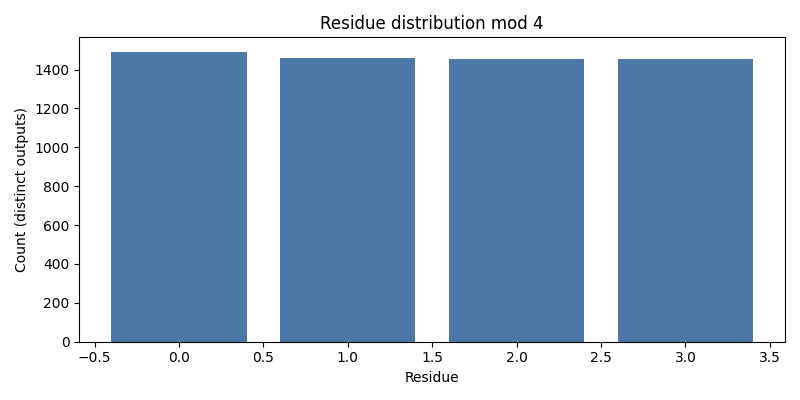
\includegraphics[width=0.7\linewidth]{../fig/residues_mod_4.png}
\caption{Residue distribution modulo 4 among distinct outputs for \(m,n\le 120\).}
\label{fig:mod4}
\end{figure}

\begin{figure}[h]
\centering
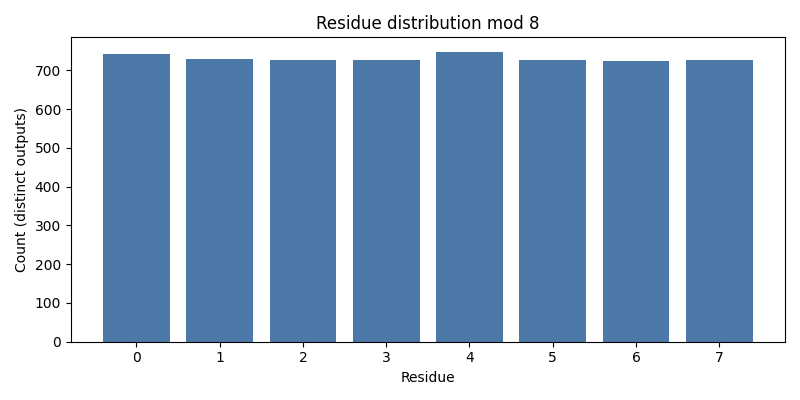
\includegraphics[width=0.7\linewidth]{../fig/residues_mod_8.png}
\caption{Residue distribution modulo 8 among distinct outputs for \(m,n\le 120\).}
\label{fig:mod8}
\end{figure}

\section{Factorization identity and coverage}
Define \(a=m+1\) and \(b=n+1\). Then
\[
F(m,n) = 4 + 3m + 3n + 2mn = 2ab + a + b,
\]
and consequently
\[
2F(m,n) + 1 = (2a+1)(2b+1) = (2m+3)(2n+3).
\]

\begin{theorem}[Odd composites via \(F\)]\label{thm:coverage}
For every odd composite integer \(c\ge 9\), there exist \(m,n\in\mathbb{N}_0\) such that \(2F(m,n) + 1 = c\). Equivalently, \(F\) parameterizes exactly the indices \(x\) with \(2x+1\) odd composite.
\end{theorem}
\begin{proof}
Write \(c=uv\) with \(u,v\) odd integers and \(3\le u\le v\). Set \(a=(u-1)/2\), \(b=(v-1)/2\), so \(a,b\in\mathbb{N}\). Let \(m=a-1\), \(n=b-1\). Then
\(2F(m,n) + 1 = (2a+1)(2b+1) = uv = c\), as claimed. Conversely, any \((m,n)\) yields \(2F(m,n)+1=(2m+3)(2n+3)\), an odd composite \(\ge 9\).
\end{proof}

\begin{corollary}[Multiplicity and collisions]\label{cor:mult}
Let \(x=F(m,n)\) and \(c=2x+1\). The number of preimages \((m,n)\) mapping to \(x\) equals the number of ordered odd factor pairs \((u,v)\) of \(c\) with \(u,v\ge 3\). In particular, squares \(c=u^2\) contribute a single ordered pair \((u,u)\), while non-squares contribute pairs \((u,v)\) and \((v,u)\), causing collisions under the cancellation scheme.
\end{corollary}

\begin{corollary}[Preimage count via odd divisors]\label{cor:odddiv}
For odd composite \(c\ge 9\), the number of ordered preimages \((m,n)\) with \(2F(m,n)+1=c\) equals \(d_{\mathrm{odd}}(c) - 2\).
\end{corollary}
\begin{proof}
Odd divisors \(u\) of \(c\) correspond to ordered pairs \((u, c/u)\). Excluding \(u=1\) and \(u=c\) leaves \(d_{\mathrm{odd}}(c)-2\) ordered pairs with components \(\ge 3\), each giving a unique \((m,n)\).
\end{proof}

\section{Related work}
The representation \(2F(m,n)+1=(2m+3)(2n+3)\) aligns with the classical parameterization of odd composites as products of odd integers. Standard references in multiplicative number theory (e.g., \cite{hardywright2008, montgomery2007}) discuss factorization structures and their combinatorics. Our contribution here is to fix a specific affine reparametrization \((m,n)\mapsto (2m+3,2n+3)\) and to study collision behavior under a cancellation rule tied to multiplicity.

\section{Discussion}
The collision-zero model encodes multiplicity within the image of \(f\). Since \(f\) does not cover all odd composites (Lemma~\ref{rem:sparse}), this model should be viewed as a structured subset rather than a complete characterization of primes or composites. Lemma~\ref{lem:mod3} explains that no simple modulo-3 obstruction limits the image to two residue classes; all three occur. Empirical comparisons to zero statistics may be framed against classical pair-correlation heuristics (e.g., \cite{montgomery1973}) and large-scale computations (e.g., \cite{odlyzko1987}).

\subsection*{Limitations}
- The collision rule is a modeling device; it compresses multiplicity but does not, by itself, imply analytic statements about primes or zeta zeros.
- The spectral or statistical behavior of the image of \(f\) is empirical here and not used to claim the Riemann Hypothesis.
- Uniqueness and density statements depend on the chosen domain rectangle for \((m,n)\); asymptotics require careful normalization.

\section{Conclusion}
We formalized and implemented the collision-zero encoding for \(f(m,n)\). The model provides a lens on multiplicity but does not, as formulated, prove statements about the zeros of \(\zeta(s)\).

\appendix
\section{Proof structure}
Assumptions: integers \(m,n\ge 0\); cancellation sets repeated images to zero. Core steps:
\begin{itemize}
  \item Algebra: \(F(m,n)=2(m{+}1)(n{+}1)+(m{+}1)+(n{+}1)\) and \(2F(m,n)+1=(2m{+}3)(2n{+}3)\).
  \item Coverage (Theorem~\ref{thm:coverage}): factor any odd composite \(c\ge 9\) as \(uv\) with odd \(u,v\ge 3\); set \(m=(u{-}3)/2\), \(n=(v{-}3)/2\).
  \item Multiplicity (Cor.~\ref{cor:mult}): preimages correspond to ordered odd factor pairs of \(2F{+}1\).
\end{itemize}

\section{Reproducibility}
Environment: Python 3.13; optional \texttt{sympy} for primality. Commands:
\begin{lstlisting}[language=bash]
# Residue/distribution profiles (example bounds)
python3 python/true_string_collision.py --max-m 120 --max-n 120 \
  --mods 3,4,8 --divisible-by 2,3,5,7,11

# Coverage test: every odd composite c >= 9 is 2*F(m,n)+1
python3 python/test_parametric_odd_composites.py 200000

# Multiplicity test: compare preimage counts to d_odd(c)-2 on a sample
python3 python/verify_multiplicity.py 200000
\end{lstlisting}

\bibliographystyle{plain}
\bibliography{references}

\end{document}